\section{Circuitos secuenciales}

Aunque hemos comentado con profusión los circuitos combinacionales, lo que realmente impera en la práctica son los circuitos secuenciales. Mientras que hemos visto que en los circuitos combinacionales la salida depende exclusivamente de los valores de las entradas en el momento actual, en los circuitos secuenciales se tienen los valores de las entradas en el pasado. Por ejemplo, si tenemos un ventilador con diferentes velocidades y queremos aumentarla, tenemos que saber algo más aparte de una entrada que indique el incremento de la velocidad. Es decir, tendría que haber un estado que nos indique la velocidad actual del sistema para saber cómo incrementar la velocidad. Es aquí donde entran en juego las \emph{máquinas de estado.}

\subsection{Máquinas de estado.}

El funcionamiento de un sistema como el ventilador puede ser conceptualizada como un conjunto de estados interrelacionados, es decir, una \hyperlink{state-machine}{máquina de estados.} El estado de un circuito secuencial puede definirse como ``una colección de \emph{variables de estado} cuyos valores en cualquier instante contienen toda la información acerca del pasado necesaria para predecir el comportamiento del circuito en el futuro'' \textcolor{red}{CITAR LIBRO DE HERERT HELLERMAN DIGITAL COMPUTER SYSTEM PRINCIPLES DE 1967}. No obstante, son necesarias más cosas aparte de variables de estado, por ejemplo, se necesita saber hacia qué estado. Este no solo dependerá del valor de las entradas del sistema, sino del estado en el que se encuentre en ese momento. En el ejemplo del ventilador, si activamos la señal de incremento de la velocidad y nos encontramos en el estado \emph{VELOCIDAD\_MEDIA}, el circuito se moverá al estado \emph{VELOCIDAD\_ALTA}. Por el contrario, para la misma entrada, si el circuito se encontrara en el estado \emph{VELOCIDAD\_BAJA}, éste cambiaría a \emph{VELOCIDAD\_MEDIA}. Como el númerod de estados de un sistema no es infinito, las máquinas de estado (y los circuitos secuenciales en general) se suelen conocer también por el nombre de \emph{máquinas de estados finitos.}

En los circuitos secuenciales cobra gran importancia el \emph{reloj}, ya que los cambios entre estados deben llevarse a cabo de manera sincronizada. En la mayoría de sistemas, el cambio de estado se lleva a cabo en los \hyperlink{edge}{\emph{flancos}} del reloj, o \hyperlink{active_edge}{\emph{flancos activos/gatillo}}, ya sea de subida o de bajada (aunque es más frecuente en el de subida). Una señal de reloj es \hyperlink{active_high}{\emph{activa en alto}} si los cambios de estado se producen en el flanco de subida, o \hyperlink{active_low}{\emph{activa en bajo}} si los cambios se llevan a cabo en el flanco de bajada. Este tipo de relojes debe estár activo, funcionando a una frecuencia dada y regular, mientras el circuito esté activo. Esta señal de reloj con frecuencia es generada por un oscilador de cristal de cuarzo, cuya frecuencia varía dependiendo del circuito en el que se integre.

Otro elemento a tener en cuenta en los circuitos secuenciales es el de \hyperlink{flip-flop}{biestable}. Estos son elementos con memoria, que permiten mantener el valor de las variables de estado, entre otras cosas. Un biestable se puede implementar por medio de un \hyperlink{feedback_sequential_circuit}{\emph{circuito secuencial retroalimentado}}, en el cual un bucle de retroalimentación se incluye en el circuito secuencial para añadir memoria al sistema. Hay multitud de tipos de biestables:

\begin{itemize}
    \item \emph{Biestable SR.}
    \item \emph{Biestable JK.}
    \item \emph{Biestable D.}
    \item \emph{Biestable T.}
\end{itemize}

\subsubsection{Estructura de las máquinas de estado}

La mayoría de máquinas de estado actuales son \hyperlink{clocked_synchronous_state_machine}{\emph{máquinas de estado sincronizadas por reloj}} que usan biestables D disparados por flanco. Son sincronizados por reloj porque todos los biestables están conectados a la misma señal de reloj, cambiando al mismo tiempo su estado en respuesta a los flancos del reloj. Las Figuras \ref{fig:mef-mealy} y \ref{fig:mef-moore} muestran la estructura general de una máquina de estados finitos de Mealy y de Moore, respectivamente. Ambas tienen en común una \emph{memoria de estado}, que está constituida por un conjunto de $n$ biestables que almacenan el estado del circuito. A estos biestables se les conecta una \emph{señal de reloj} común, the tal manera que el estado sólo cambia en los \emph{tics} del reloj. El \emph{tic} (se podría definir como el instante en el que cambia el estado) depende del tipo de biestable usado. Por ejemplo, para los biestables que se activan en el flanco de subida, el tic es el flanco de subida del reloj. El estado siguiente de la máquina de estados viene determinado por la \emph{lógica del estado siguiente} que es función del estado actual y las entradas. En cambio, la \emph{lógica de salida} depende del tipo de circuito del que se trate. En las máquinas de estados finitos de Mealy, la lógica de salida viene determinada por las entradas y el estado actual.

\begin{figure}[h]
    \centering
    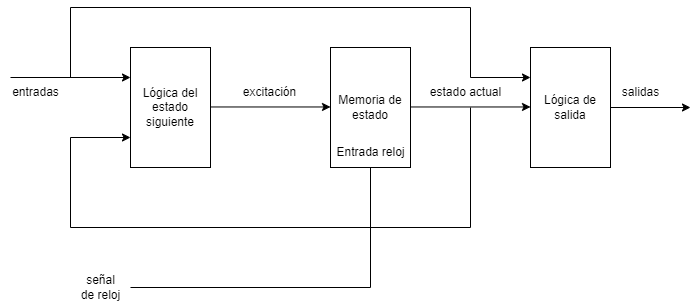
\includegraphics[width=\textwidth]{figs/mef-mealy.drawio.png}
    \caption[short]{Máquina de estados finitos de Mealy.}
    \label{fig:mef-mealy}
\end{figure}

En cambio, en una máquina de estados finitos de Moore, la lógica de salida viene determinada exclusivamente del estado actual.

\begin{figure}[h]
    \centering
    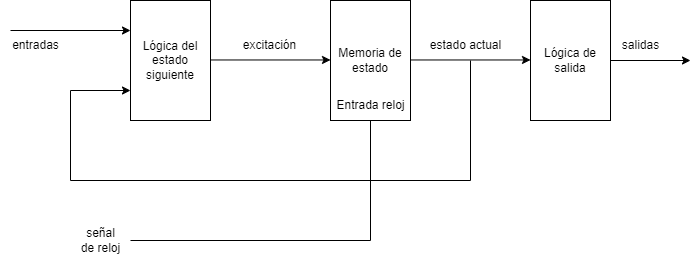
\includegraphics[width=\textwidth]{figs/mef-moore.drawio.png}
    \caption[short]{Máquina de estados finitos de Moore.}
    \label{fig:mef-moore}
\end{figure}

Como se puede observar en los diagramas, la única diferencia entre ambos tipos de modelos radica en cómo se generan las salidas. 

En el diseño de circuitos de gran velocidad es necesario que las salidas estén disponibles lo antes posible. Por ello, en ocasiones se codifican las variables de estado para que sirvan de salida también. Este tipo de diseño se denomina \hyperlink{output-coded_state_assignment}{\emph{asignación de estados codificada en salidas}}. En este caso la salida del circuito consiste en \verb|wires|. Otra manera de abordar el diseño de una máquina de estados es haciendo que la salida durante un periodo de reloj dependa de la salida en el periodo de reloj anterior. Esto se denomina \hyperlink{pipelined_outputs}{\emph{salida por etapas}} y se consigue uniendo otra etapa de memoria, llamada \emph{memoria de salida por etapas}, a las salidas del circuito.

\subsubsection{Temporización de las máquinas de estados}

\textcolor{red}{POR HACER}

\subsection{Diseño de máquinas de estado con tablas de estado}

\textcolor{red}{POR HACER (pag. 455)}

\subsection{Diseño de máquinas de estado con diagramas de estado}

\textcolor{red}{POR HACER (pag. 472)}

\subsection{Diseño de máquinas de estado con Verilog}

Para explicar el diseño de máquinas de estados vamos a partir de las siguientes especificaciones:

Diseña una máquina de estados síncrona con reloj con dos entradas, A y B, y una salida Z que es 1 si:

\begin{itemize}
    \item A tiene el mismo valor que en los dos tics de reloj previos.
    \item B vale uno tras la última vez que la primera condición fue cierta.
\end{itemize}

Si las condiciones no se cumplen, Z vale 0.

Para visualizar mejor estas condiciones, lo mejor es comenzar describiendo una tabla de estados y salidas. La Tabla \ref{tab:tabla-salidas-estados} muestra el resultado sobre el cual vamos a trabajar para escribir el código en Verilog.

\begin{table}
    \centering
    \begin{tblr}{
      row{2} = {c},
      row{3} = {c},
      row{4} = {c},
      row{5} = {c},
      row{6} = {c},
      row{7} = {c},
      cell{1}{2} = {c=4}{c},
      cell{8}{2} = {c=5}{c},
      hline{1,9} = {-}{},
      hline{2} = {2-5}{},
      hline{8} = {2-6}{},
    }
                        & \textbf{\textit{AB}} &                      &                      &                      &                     \\
    \textbf{\textit{S}} & \textbf{\textit{00}} & \textbf{\textit{01}} & \textbf{\textit{11}} & \textbf{\textit{10}} & \textbf{\textit{Z}} \\
    INIT                & A0                   & A0                   & A1                   & A1                   & 0                   \\
    A0                  & OK0                  & OK0                  & A1                   & A1                   & 0                   \\
    A1                  & A0                   & A0                   & OK1                  & OK1                  & 0                   \\
    OK0                 & OK0                  & OK0                  & OK1                  & A1                   & 1                   \\
    OK1                 & A0                   & OK0                  & OK1                  & OK1                  & 1                   \\
                        & S*                   &                      &                      &                      &                     
    \end{tblr}

    \caption{Tabla de salidas y estados}
    \label{tab:tabla-salidas-estados}
    \end{table}

El correspondiente módulo en Verilog se compondrá de cinco secciones:

\begin{enumerate}
    \item La declaración de las entradas, salidas y variables internas al módulo.
    \item Sentencias \verb|parameter| para asignar las variables de estado a su nombre.
    \item Un primer bloque \verb|always| para crear la memoria de estado.
    \item Un segundo bloque \verb|always| para definir el comportamiento del estado siguiente.
    \item Un tercer bloque \verb|always| para definir la lógica de salida.
\end{enumerate}

El código en Verilog resultante se muestra en el Listing \ref{lst:maquina-estado-verilog}.

\begin{mycode}[style=verilogstyle, caption={Máquina de estado en Verilog.}, label=lst:maquina-estado-verilog]
module mef (
            // reloj y reset
            input clk,
            input rst,

            // entradas
            input A,
            intput B,

            // salidas (como vamos a usar codigo procedural, hay que declarar la salida como reg)
            output reg Z
           );

// senales internas
reg estado, estado_siguiente;

// asignacion de variables de estado a parametros
parameter [2:0] INIT = 3'b000;
                A0 = 3'b001;
                A1 = 3'b010;
                OK0 = 3'b011;
                OK1 = 3'b100;

// comportamiento del estado siguiente
always @(*) begin
    case(estado)
        INIT: if (A == 0) estado_siguiente = A0;
              else estado_siguiente = A1;
        A0: if (A == 0) estado_siguiente = OK0;
            else estado_siguiente = A1;
        A1: if (A == 0) estado_siguiente = A0;
            else estado_siguiente = OK1;
        OK0: if (A == 0) estado_siguiente = OK0;
             else if ((A == 0) && (B == 1)) estado_siguiente = OK1;
             else estado_siguiente = A1;
        OK1: if ((A == 0) && (B == 0)) estado_siguiente = A0;
        else if ((A == 0) && (B == 1)) estado_siguiente = OK0;
        else estado_siguiente = OK1;
        default: estado_siguiente = INIT;
    endcase
end

// logica de salida
always @(estado) begin
    case(estado)
        INIT: Z = 0;
        A0: Z = 0;
        A1: Z = 0;
        OK0: Z = 1;
        OK1: Z = 1;
        default: Z = 0;
    endcase
end

// memoria de estado
always @(posedge clk) begin
    if(rst)
        estado <= 0;
    else
        estado <= estado_siguiente;
end

\end{mycode}